\documentclass{article}
\usepackage{amssymb}
\usepackage{amsmath}
\usepackage{tikz}
\usepackage{pdfpages}
\usepackage{enumitem}
\newlist{alphalist}{enumerate}{1}
\setlist[alphalist,1]{label=\textbf{\Alph*.}}


\usepackage{listings}
\usepackage{color}


\begin{document}

\begin{flushleft}
  Eli Schmitter\\
  \today
\end{flushleft}
\section{}
\begin{alphalist}
  \item A binary tree is a data structurer where each node has a parent node(except for the root node) and at most two children node.
  \item the root is the first node on a tree.
  \item a leaf is a node that has two null children
  \item a sub tree is a tree of a that has its root node as a child node in another tree
  \item siblings are nodes that are on the same level of the tree
  \item parent the node that has children
  \item a node that can get to from a parent
  \item the number of arguments a function takes.
  \item a node with at least one child node.
\end{alphalist}
\section{}
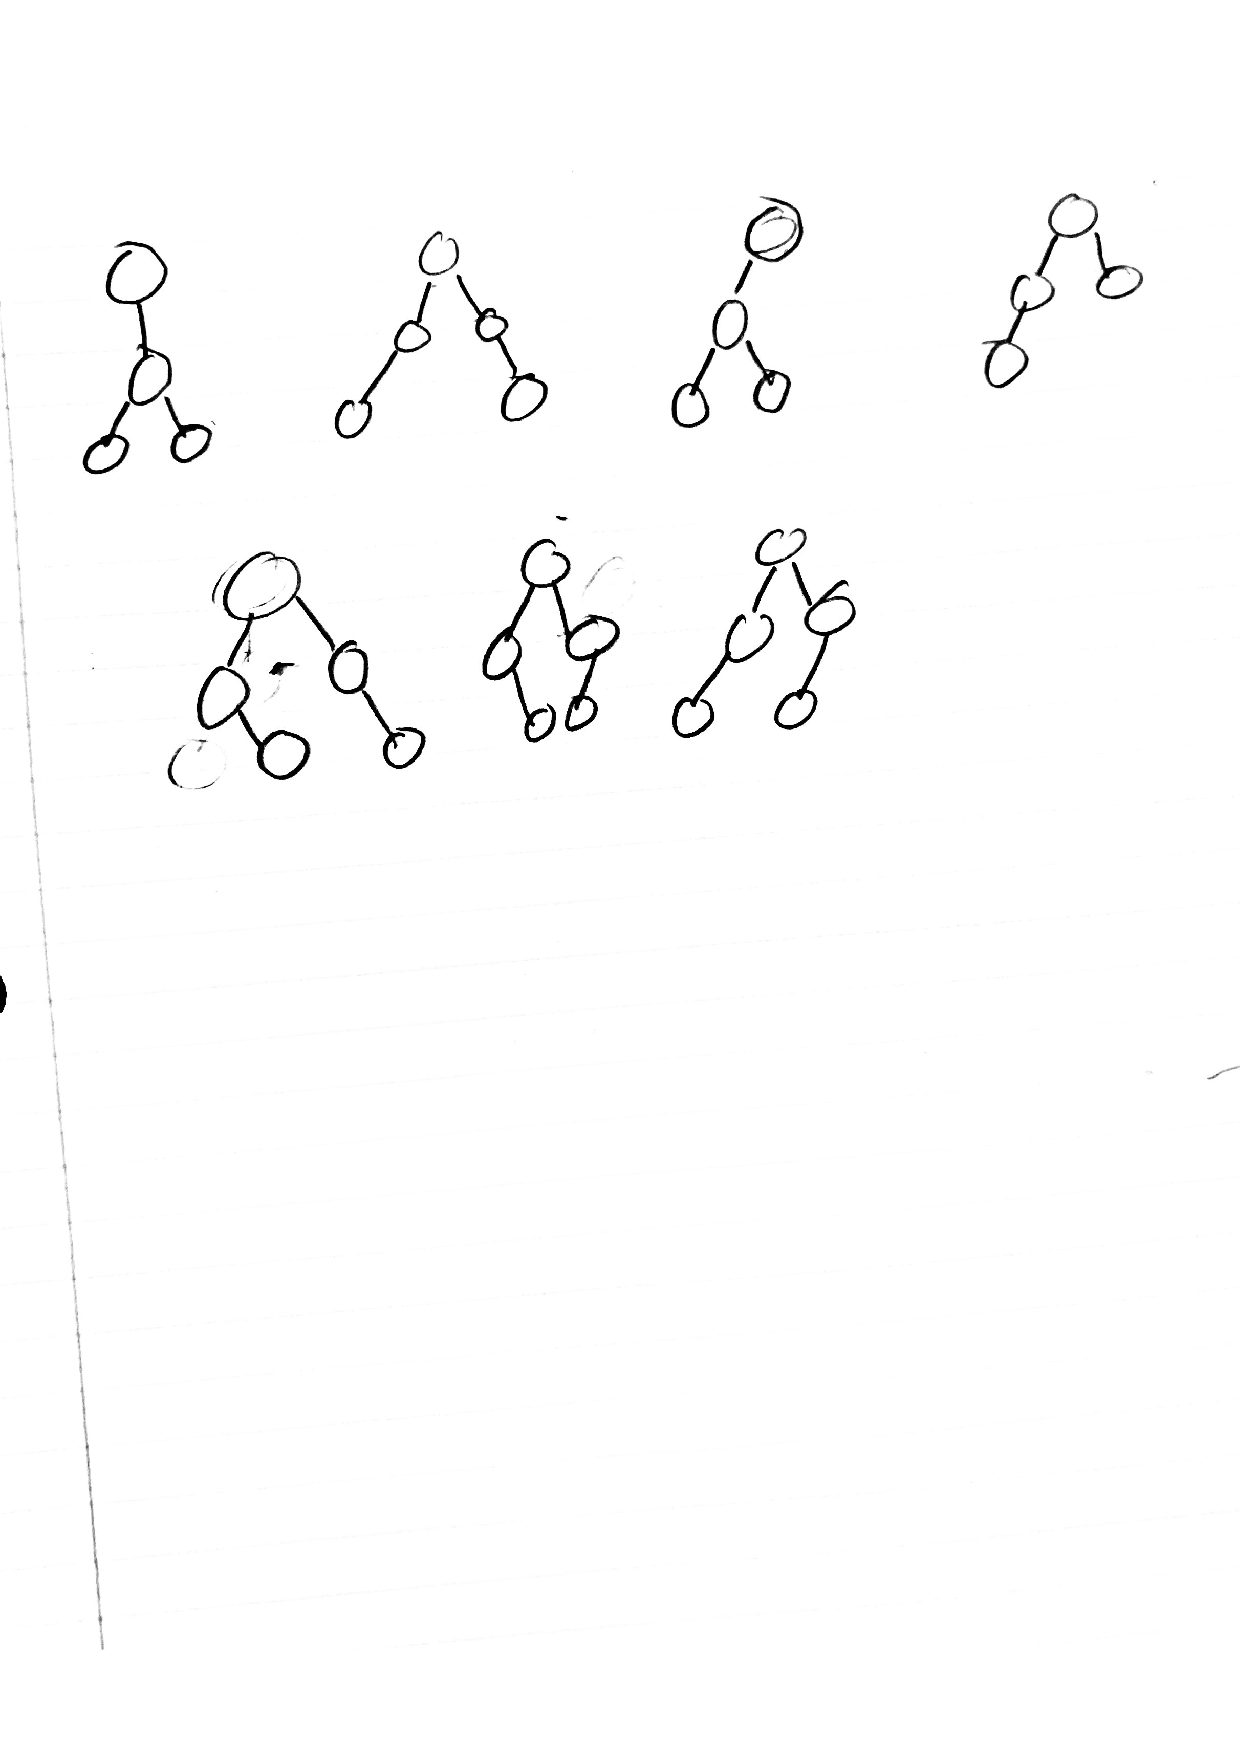
\includepdf{nodes}
\section{R17.4}
if there is at least two leafs then there has to be at least one parent node for two children. This goes recursively back to the root. 
\section{R17.1}
A binary tree is a unordered where a binary search tree is ordered. The binary search tree is used for searching because the order makes it faster.
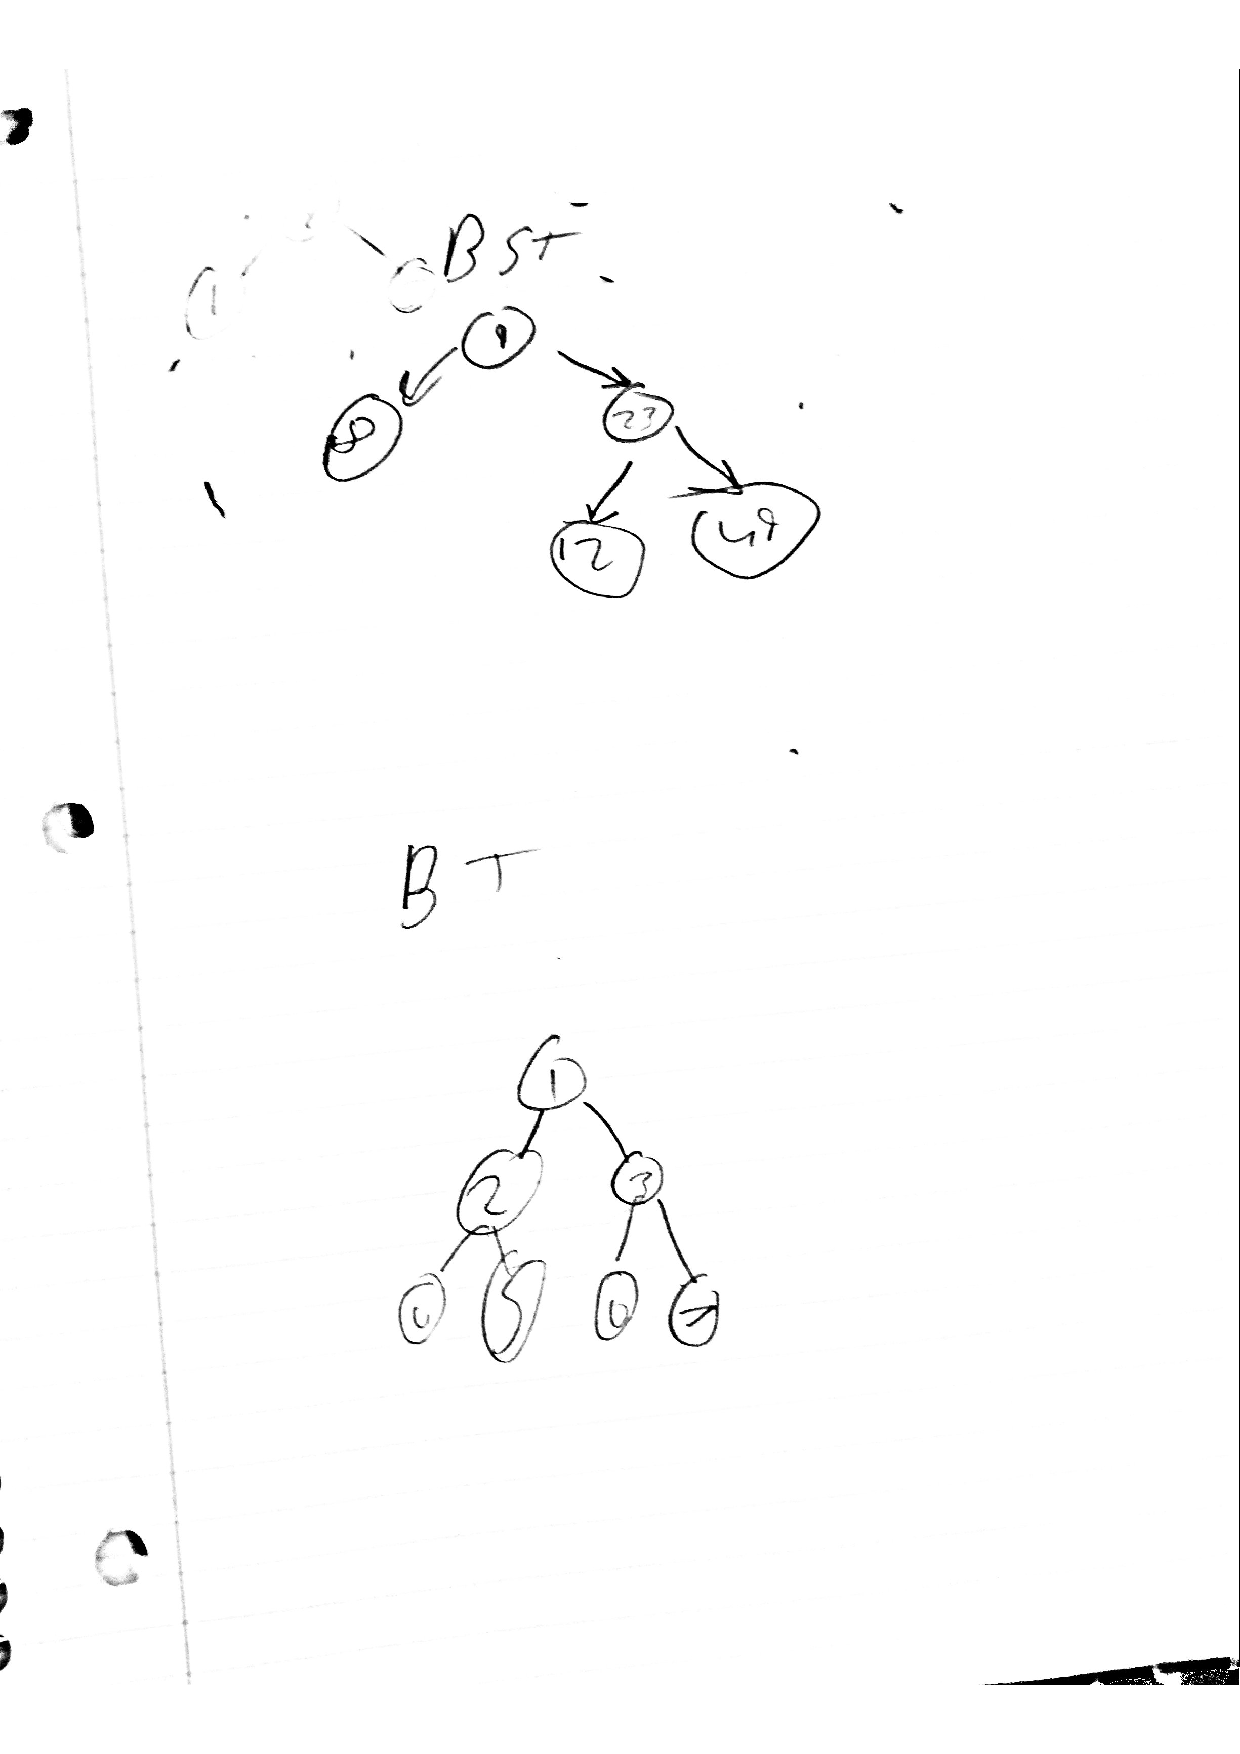
\includepdf{bst}
\section{R17.10}
\begin{enumerate}
\item start at root
\item move down the leftmost node
\item if  k == i then thats k, i is the number of iterations.
\item else move up one
\item i++
\item if a right childed node is there go down it
\item go to 2
\end{enumerate}
\section{E17.1}
\begin{lstlisting}[language=java]
    public int count(BinaryTree b){
        if (b==null){
            return 0;
        }
        if(b.isLeaf()){
            return 1;
        }
        return  count(b.getLeftChild())+count(b.getRightChild());
    }
\end{lstlisting}
\end{document}
